\documentclass[]{article}
\usepackage{lmodern}
\usepackage{amssymb,amsmath}
\usepackage{ifxetex,ifluatex}
\usepackage{fixltx2e} % provides \textsubscript
\ifnum 0\ifxetex 1\fi\ifluatex 1\fi=0 % if pdftex
  \usepackage[T1]{fontenc}
  \usepackage[utf8]{inputenc}
\else % if luatex or xelatex
  \ifxetex
    \usepackage{mathspec}
  \else
    \usepackage{fontspec}
  \fi
  \defaultfontfeatures{Ligatures=TeX,Scale=MatchLowercase}
\fi
% use upquote if available, for straight quotes in verbatim environments
\IfFileExists{upquote.sty}{\usepackage{upquote}}{}
% use microtype if available
\IfFileExists{microtype.sty}{%
\usepackage{microtype}
\UseMicrotypeSet[protrusion]{basicmath} % disable protrusion for tt fonts
}{}
\usepackage[margin=1in]{geometry}
\usepackage{hyperref}
\hypersetup{unicode=true,
            pdftitle={Laborator 2},
            pdfborder={0 0 0},
            breaklinks=true}
\urlstyle{same}  % don't use monospace font for urls
\usepackage{color}
\usepackage{fancyvrb}
\newcommand{\VerbBar}{|}
\newcommand{\VERB}{\Verb[commandchars=\\\{\}]}
\DefineVerbatimEnvironment{Highlighting}{Verbatim}{commandchars=\\\{\}}
% Add ',fontsize=\small' for more characters per line
\usepackage{framed}
\definecolor{shadecolor}{RGB}{248,248,248}
\newenvironment{Shaded}{\begin{snugshade}}{\end{snugshade}}
\newcommand{\KeywordTok}[1]{\textcolor[rgb]{0.13,0.29,0.53}{\textbf{#1}}}
\newcommand{\DataTypeTok}[1]{\textcolor[rgb]{0.13,0.29,0.53}{#1}}
\newcommand{\DecValTok}[1]{\textcolor[rgb]{0.00,0.00,0.81}{#1}}
\newcommand{\BaseNTok}[1]{\textcolor[rgb]{0.00,0.00,0.81}{#1}}
\newcommand{\FloatTok}[1]{\textcolor[rgb]{0.00,0.00,0.81}{#1}}
\newcommand{\ConstantTok}[1]{\textcolor[rgb]{0.00,0.00,0.00}{#1}}
\newcommand{\CharTok}[1]{\textcolor[rgb]{0.31,0.60,0.02}{#1}}
\newcommand{\SpecialCharTok}[1]{\textcolor[rgb]{0.00,0.00,0.00}{#1}}
\newcommand{\StringTok}[1]{\textcolor[rgb]{0.31,0.60,0.02}{#1}}
\newcommand{\VerbatimStringTok}[1]{\textcolor[rgb]{0.31,0.60,0.02}{#1}}
\newcommand{\SpecialStringTok}[1]{\textcolor[rgb]{0.31,0.60,0.02}{#1}}
\newcommand{\ImportTok}[1]{#1}
\newcommand{\CommentTok}[1]{\textcolor[rgb]{0.56,0.35,0.01}{\textit{#1}}}
\newcommand{\DocumentationTok}[1]{\textcolor[rgb]{0.56,0.35,0.01}{\textbf{\textit{#1}}}}
\newcommand{\AnnotationTok}[1]{\textcolor[rgb]{0.56,0.35,0.01}{\textbf{\textit{#1}}}}
\newcommand{\CommentVarTok}[1]{\textcolor[rgb]{0.56,0.35,0.01}{\textbf{\textit{#1}}}}
\newcommand{\OtherTok}[1]{\textcolor[rgb]{0.56,0.35,0.01}{#1}}
\newcommand{\FunctionTok}[1]{\textcolor[rgb]{0.00,0.00,0.00}{#1}}
\newcommand{\VariableTok}[1]{\textcolor[rgb]{0.00,0.00,0.00}{#1}}
\newcommand{\ControlFlowTok}[1]{\textcolor[rgb]{0.13,0.29,0.53}{\textbf{#1}}}
\newcommand{\OperatorTok}[1]{\textcolor[rgb]{0.81,0.36,0.00}{\textbf{#1}}}
\newcommand{\BuiltInTok}[1]{#1}
\newcommand{\ExtensionTok}[1]{#1}
\newcommand{\PreprocessorTok}[1]{\textcolor[rgb]{0.56,0.35,0.01}{\textit{#1}}}
\newcommand{\AttributeTok}[1]{\textcolor[rgb]{0.77,0.63,0.00}{#1}}
\newcommand{\RegionMarkerTok}[1]{#1}
\newcommand{\InformationTok}[1]{\textcolor[rgb]{0.56,0.35,0.01}{\textbf{\textit{#1}}}}
\newcommand{\WarningTok}[1]{\textcolor[rgb]{0.56,0.35,0.01}{\textbf{\textit{#1}}}}
\newcommand{\AlertTok}[1]{\textcolor[rgb]{0.94,0.16,0.16}{#1}}
\newcommand{\ErrorTok}[1]{\textcolor[rgb]{0.64,0.00,0.00}{\textbf{#1}}}
\newcommand{\NormalTok}[1]{#1}
\usepackage{longtable,booktabs}
\usepackage{graphicx,grffile}
\makeatletter
\def\maxwidth{\ifdim\Gin@nat@width>\linewidth\linewidth\else\Gin@nat@width\fi}
\def\maxheight{\ifdim\Gin@nat@height>\textheight\textheight\else\Gin@nat@height\fi}
\makeatother
% Scale images if necessary, so that they will not overflow the page
% margins by default, and it is still possible to overwrite the defaults
% using explicit options in \includegraphics[width, height, ...]{}
\setkeys{Gin}{width=\maxwidth,height=\maxheight,keepaspectratio}
\IfFileExists{parskip.sty}{%
\usepackage{parskip}
}{% else
\setlength{\parindent}{0pt}
\setlength{\parskip}{6pt plus 2pt minus 1pt}
}
\setlength{\emergencystretch}{3em}  % prevent overfull lines
\providecommand{\tightlist}{%
  \setlength{\itemsep}{0pt}\setlength{\parskip}{0pt}}
\setcounter{secnumdepth}{5}
% Redefines (sub)paragraphs to behave more like sections
\ifx\paragraph\undefined\else
\let\oldparagraph\paragraph
\renewcommand{\paragraph}[1]{\oldparagraph{#1}\mbox{}}
\fi
\ifx\subparagraph\undefined\else
\let\oldsubparagraph\subparagraph
\renewcommand{\subparagraph}[1]{\oldsubparagraph{#1}\mbox{}}
\fi

%%% Use protect on footnotes to avoid problems with footnotes in titles
\let\rmarkdownfootnote\footnote%
\def\footnote{\protect\rmarkdownfootnote}

%%% Change title format to be more compact
\usepackage{titling}

% Create subtitle command for use in maketitle
\newcommand{\subtitle}[1]{
  \posttitle{
    \begin{center}\large#1\end{center}
    }
}

\setlength{\droptitle}{-2em}
  \title{Laborator 2}
  \pretitle{\vspace{\droptitle}\centering\huge}
  \posttitle{\par}
\subtitle{Elemente de statistică descriptivă și exploratorie}
  \author{}
  \preauthor{}\postauthor{}
  \date{}
  \predate{}\postdate{}

\usepackage{booktabs}
\usepackage{longtable}
\usepackage{framed,color}
\definecolor{shadecolor}{RGB}{248, 248, 248}
%\definecolor{shadecolor1}{RGB}{216,225,235}
%\definecolor{framecolor}{RGB}{108,123,13}

%\definecolor{shadecolor}{RGB}{226, 255, 241}
\definecolor{shadecolor1}{RGB}{217,225,199}
\definecolor{framecolor}{RGB}{60,179,113}

\ifxetex
  \usepackage{letltxmacro}
  \setlength{\XeTeXLinkMargin}{1pt}
  \LetLtxMacro\SavedIncludeGraphics\includegraphics
  \def\includegraphics#1#{% #1 catches optional stuff (star/opt. arg.)
    \IncludeGraphicsAux{#1}%
  }%
  \newcommand*{\IncludeGraphicsAux}[2]{%
    \XeTeXLinkBox{%
      \SavedIncludeGraphics#1{#2}%
    }%
  }%
\fi

\newenvironment{frshaded*}{%
  \def\FrameCommand{\fboxrule=\FrameRule\fboxsep=\FrameSep \fcolorbox{framecolor}{shadecolor1}}%
  \MakeFramed {\advance\hsize-\width \FrameRestore}}%
{\endMakeFramed}

\newenvironment{rmdblock}[1]
  {\begin{frshaded*}
  \begin{itemize}
  \renewcommand{\labelitemi}{
    \raisebox{-.7\height}[0pt][0pt]{
      {\setkeys{Gin}{width=2em,keepaspectratio}\includegraphics{images/icons/#1}}
    }
  }
  \item
  }
  {
  \end{itemize}
  \end{frshaded*}
  }

\newenvironment{rmdcaution}
  {\begin{rmdblock}{caution}}
  {\end{rmdblock}}
% \newenvironment{rmdinsight}
%   {\begin{rmdblock}{insight}}
%   {\end{rmdblock}}
\newenvironment{rmdexercise}
  {\begin{rmdblock}{exercise}}
  {\end{rmdblock}}
\newenvironment{rmdtip}
  {\begin{rmdblock}{tip}}
  {\end{rmdblock}}


%%%%%%%%%%%%%%%%%%%%%%%%%%%%%%%%%%%%%%%%%%%%%%%%%%%%%%%%%%%%%%%%%%%%%%%%%%%%%%%%%%%%%%%%%%%%%%%%%%%%%%%%%%%%%%%%%%%%%
%%%%%%%%%%% For insight block %%%%%%%%%%%%%%%%%%%%%%%%%%
\definecolor{shadecolor_insight}{RGB}{223,240,216}
\definecolor{framecolor_insight}{RGB}{136,193,137}

%\definecolor{shadecolor_insight}{RGB}{217,225,199}
%\definecolor{framecolor_insight}{RGB}{60,179,113}

\newenvironment{frshaded_insight*}{%
  \def\FrameCommand{\fboxrule=\FrameRule\fboxsep=\FrameSep \fcolorbox{framecolor_insight}{shadecolor_insight}}%
  \MakeFramed {\advance\hsize-\width \FrameRestore}}%
{\endMakeFramed}

\newenvironment{rmdblock_insight}[1]
  {\begin{frshaded_insight*}
  \begin{itemize}
  \renewcommand{\labelitemi}{
    \raisebox{-.7\height}[0pt][0pt]{
      {\setkeys{Gin}{width=2em,keepaspectratio}\includegraphics{images/icons/#1}}
    }
  }
  \item
  }
  {
  \end{itemize}
  \end{frshaded_insight*}
  }

\newenvironment{rmdinsight}
  {\begin{rmdblock_insight}{insight}}
  {\end{rmdblock_insight}}

%%%%%%%%%%%%%%%%%%%%%%%%%%%%%%%%%%%%%%%%%%%%%%%%%%%%%%%%%%%%%%%%%%%%%%%%%%%%%%%%%%%%%%%%%%%%%%%%%%%%%%%%%%%%%%%%%%%%%
\usepackage{subfigure}
\usepackage{booktabs}
\usepackage{slashbox}
\usepackage{color}
%%%%%%%%%%%%%%%%%%%%%%%%%%%%%%%%%%%%%%%%%%%%%%%%%%%%%%%%%%%%%%%%%%%%%%%%%%%%%%%%%%%%%%%%%%%%%%%%%%%%%%%%%%%%%%%%%%%%%
%CITEVA DEFINITII
\def\om{\omega}
\def\Om{\Omega}
\def\et{\eta}
\def\td{\tilde{\delta}}
\def\m{{\mu}}
\def\n{{\nu}}
\def\k{{\kappa}}
\def\l{{\lambda}}
\def\L{{\Lambda}}
\def\g{{\gamma}}
\def\a{{\alpha}}
\def\e{{\varepsilon}}
\def\b{{\beta}}
\def\G{{\Gamma}}
\def\d{{\delta}}
\def\D{{\Delta}}
\def\t{{\theta}}
\def\s{{\sigma}}
\def\S{{\Sigma}}
\def\z{{\zeta}}
\def\qed{\hfill\Box}
\def\ds{\displaystyle}
\def\mc{\mathcal}
%%%%%%%%%%%%%%%%%%%%%%%%%%%%%%%%%%%%%%%%%%%%%%%%%%%%%%%%%%%%%%%%%%%%%%%%%%%%%%%%%%%%%%%%%%%%%%%%%%%%%%%%%%%%%%%%%%%%%%
\def\1{{\mathbf 1}}
\def\CC{{\mathbb C}}
\def\VV{{\mathbb V}}
\def\RR{{\mathbb R}}
\def\QQ{{\mathbb Q}}
\def\ZZ{{\mathbb Z}}
\def\PP{{\mathbb P}}
\def\EE{{\mathbb E}}
\def\NN{{\mathbb N}}
\def\FF{{\mathbb F}}
%\def\SS{{\mathbb S}}
\def\MA{{\mathcal A}}
\def\MO{{\mathcal O}}
\def\MF{{\mathcal F}}
\def\ME{{\mathcal E}}
\def\MR{{\mathcal R}}
\def\MB{{\mathcal B}}
\def\MM{{\mathcal M}}
\def\MN{{\mathcal N}}
\def\MU{{\mathcal U}}
\def\MP{{\mathcal P}}
\def\MS{{\mathcal S}}
\def\MBS{{\mathbf S}}
\def\MX{{\bm{ \mathscr X}}}

% independent sign
\newcommand\independent{\protect\mathpalette{\protect\independenT}{\perp}}
\def\independenT#1#2{\mathrel{\rlap{$#1#2$}\mkern2mu{#1#2}}}

\renewcommand\tablename{Tab.}
\renewcommand{\figurename}{Fig.}
\renewcommand\refname{Referințe}

%%%%%%%%%%%%%%%%%%%%%%%%%%%%%%%%%%%%%%%%%%%%%%%%%%%%%%%%%%%%%%%%%%%%%%%%%%%%%%%%%%%%%%%%%%%%%%%%%%%%%%%%%%%%%%%%%%%%%
%Header and Footer
\usepackage{fancyhdr}

\pagestyle{fancy}
\fancyhf{}
\rhead{Universitatea din Bucure\c sti\\ Facultatea de Matematic\u a \c si Informatic\u a}
\lhead{\textit{Curs}: Biostatistic\u a 2018\\ \textit{Instructor}: A. Am\u arioarei}
\rfoot{Pagina \thepage}
\lfoot{Grupa: 503}
%%%%%%%%%%%%%%%%%%%%%%%%%%%%%%%%%%%%%%%
\usepackage{booktabs}
\usepackage{longtable}
\usepackage{array}
\usepackage{multirow}
\usepackage[table]{xcolor}
\usepackage{wrapfig}
\usepackage{float}
\usepackage{colortbl}
\usepackage{pdflscape}
\usepackage{tabu}
\usepackage{threeparttable}
\usepackage[normalem]{ulem}

\begin{document}
\maketitle

%%%%%%%%%%%%%%%%%%%%%%%%
\thispagestyle{fancy}

Obiectivul acestui laborator este de a prezenta câteva elemnte de
statistică descriptivă și exploratorie.

\section{Descrierea datelor}\label{descrierea-datelor}

De cele mai multe ori într-o analiză statistică ne confruntăm cu un set
de date în formă brută. Prima etapă a analizei este de a înțelege
proveniența, conținutul (ce reprezintă) și structura datelor și, în
funcție de natura analizei pe care dorim să o efectuăm, de a le aduce la
forma dorită pentru analiză (această etapă se numește etapa de
preprocesare și de obicei ocupă o parte semnificativă din analiză). De
cele mai multe ori ne dorim ca datele să fie stocate sub forma unui
tablou bidimensional (\texttt{data.frame}) cu variabilele pe coloane și
observațiile pe linii (acest tip de dată se numește
\texttt{tidy\ data}).

\begin{itemize}
\tightlist
\item
  variabile cantitative: continue (vârsta, greutateam, înălțimea, etc.)
  și discrete (pot lua un număr limitat de valori: număr de persoane
  care au participat la test, etc.)
\item
  variabile categorice: nominale (culoarea ochilor, a părului, etc.) și
  ordinale (dificultatea examenului: scăzută, medie, ridicată)
\end{itemize}

Să considerăm setul de date \texttt{chickwts} (prin apelarea funcției
\texttt{data()} puteți vedea care sunt seturile de date disponibile în
sesiunea curentă). Acest set de date include informații despre greutatea
a 71 de găini în funcție de diferite tipuri de hrănire.

\begin{Shaded}
\begin{Highlighting}[]
\CommentTok{# structura }
\KeywordTok{str}\NormalTok{(chickwts)}
\StringTok{'data.frame'}\OperatorTok{:}\StringTok{   }\DecValTok{71}\NormalTok{ obs. of  }\DecValTok{2}\NormalTok{ variables}\OperatorTok{:}
\StringTok{ }\ErrorTok{$}\StringTok{ }\NormalTok{weight}\OperatorTok{:}\StringTok{ }\NormalTok{num  }\DecValTok{179} \DecValTok{160} \DecValTok{136} \DecValTok{227} \DecValTok{217} \DecValTok{168} \DecValTok{108} \DecValTok{124} \DecValTok{143} \DecValTok{140}\NormalTok{ ...}
 \OperatorTok{$}\StringTok{ }\NormalTok{feed  }\OperatorTok{:}\StringTok{ }\NormalTok{Factor w}\OperatorTok{/}\StringTok{ }\DecValTok{6}\NormalTok{ levels }\StringTok{"casein"}\NormalTok{,}\StringTok{"horsebean"}\NormalTok{,..}\OperatorTok{:}\StringTok{ }\DecValTok{2} \DecValTok{2} \DecValTok{2} \DecValTok{2} \DecValTok{2} \DecValTok{2} \DecValTok{2} \DecValTok{2} \DecValTok{2} \DecValTok{2}\NormalTok{ ...}

\CommentTok{# primele si ultimele observatii}
\KeywordTok{head}\NormalTok{(chickwts)}
\NormalTok{  weight      feed}
\DecValTok{1}    \DecValTok{179}\NormalTok{ horsebean}
\DecValTok{2}    \DecValTok{160}\NormalTok{ horsebean}
\DecValTok{3}    \DecValTok{136}\NormalTok{ horsebean}
\DecValTok{4}    \DecValTok{227}\NormalTok{ horsebean}
\DecValTok{5}    \DecValTok{217}\NormalTok{ horsebean}
\DecValTok{6}    \DecValTok{168}\NormalTok{ horsebean}
\KeywordTok{tail}\NormalTok{(chickwts)}
\NormalTok{   weight   feed}
\DecValTok{66}    \DecValTok{352}\NormalTok{ casein}
\DecValTok{67}    \DecValTok{359}\NormalTok{ casein}
\DecValTok{68}    \DecValTok{216}\NormalTok{ casein}
\DecValTok{69}    \DecValTok{222}\NormalTok{ casein}
\DecValTok{70}    \DecValTok{283}\NormalTok{ casein}
\DecValTok{71}    \DecValTok{332}\NormalTok{ casein}
\end{Highlighting}
\end{Shaded}

\section{Măsuri de centralitate: media, mediana și
modul}\label{masuri-de-centralitate-media-mediana-si-modul}

\subsection{Media}\label{media}

Media eșantionului este considerată ca fiind punctul central care
balansează colecția de observații și se calculează după formula

\[
  \bar{X}_n = \frac{X_1+X_2+\cdots +X_n}{n}
\]

\begin{Shaded}
\begin{Highlighting}[]
\NormalTok{x.bar =}\StringTok{ }\KeywordTok{mean}\NormalTok{(chickwts}\OperatorTok{$}\NormalTok{weight)}
\NormalTok{x.bar.horsebean =}\StringTok{ }\KeywordTok{mean}\NormalTok{(chickwts}\OperatorTok{$}\NormalTok{weight[chickwts}\OperatorTok{$}\NormalTok{feed }\OperatorTok{==}\StringTok{ "horsebean"}\NormalTok{])}

\KeywordTok{mean}\NormalTok{(chickwts}\OperatorTok{$}\NormalTok{weight[chickwts}\OperatorTok{$}\NormalTok{feed}\OperatorTok{==}\StringTok{"casein"}\NormalTok{])}
\NormalTok{[}\DecValTok{1}\NormalTok{] }\FloatTok{323.5833}
\KeywordTok{mean}\NormalTok{(chickwts}\OperatorTok{$}\NormalTok{weight[chickwts}\OperatorTok{$}\NormalTok{feed}\OperatorTok{==}\StringTok{"linseed"}\NormalTok{])}
\NormalTok{[}\DecValTok{1}\NormalTok{] }\FloatTok{218.75}
\KeywordTok{mean}\NormalTok{(chickwts}\OperatorTok{$}\NormalTok{weight[chickwts}\OperatorTok{$}\NormalTok{feed}\OperatorTok{==}\StringTok{"meatmeal"}\NormalTok{])}
\NormalTok{[}\DecValTok{1}\NormalTok{] }\FloatTok{276.9091}
\KeywordTok{mean}\NormalTok{(chickwts}\OperatorTok{$}\NormalTok{weight[chickwts}\OperatorTok{$}\NormalTok{feed}\OperatorTok{==}\StringTok{"soybean"}\NormalTok{])}
\NormalTok{[}\DecValTok{1}\NormalTok{] }\FloatTok{246.4286}
\KeywordTok{mean}\NormalTok{(chickwts}\OperatorTok{$}\NormalTok{weight[chickwts}\OperatorTok{$}\NormalTok{feed}\OperatorTok{==}\StringTok{"sunflower"}\NormalTok{])}
\NormalTok{[}\DecValTok{1}\NormalTok{] }\FloatTok{328.9167}
\end{Highlighting}
\end{Shaded}

\subsection{Mediana}\label{mediana}

Mediana este acea valoare pentru care aproximativ \(50\%\) dintre
observații sunt mai mici și \(50\%\) dintre observații sunt mai mari, se
mai numește și magnitudinea de mijloc a obsevațiilor. Mediana (empirică)
se găsește cu ajutorul formulei

\[
  M_n = \left\{\begin{array}{ll}
      X_{\left(\frac{n+1}{2}\right)}, & \text{$n$ este impar}\\
      \frac{X_{\left(\frac{n}{2}\right)} + X_{\left(\frac{n}{2}+1\right)}}{2}, & \text{$n$ este par}
  \end{array}\right.
\]

unde \(X_{(i)}\) este a \(i\)-a cea mai mică observație a eșantionului
\(X_1, X_2, \ldots, X_n\) (statistica de ordine de rang \(i\)). A se
vedea sectiunea \protect\hyperlink{sec:cuantile}{Cuantile teoretice}.

\begin{Shaded}
\begin{Highlighting}[]
\NormalTok{M.bar =}\StringTok{ }\KeywordTok{median}\NormalTok{(chickwts}\OperatorTok{$}\NormalTok{weight)}
\NormalTok{M.bar.horsebean =}\StringTok{ }\KeywordTok{median}\NormalTok{(chickwts}\OperatorTok{$}\NormalTok{weight[chickwts}\OperatorTok{$}\NormalTok{feed }\OperatorTok{==}\StringTok{ "horsebean"}\NormalTok{])}
\end{Highlighting}
\end{Shaded}

\subsection{Modul}\label{modul}

Modul este valoarea cea mai frecventă din setul de date. Un set de date
poate să nu aibă mod (de exemplu dacă frecvența de apariție a
observațiilor este 1 - toate apar o singură dată), să aibă un mod, două
moduri (set bimodal) sau mai multe.

\begin{Shaded}
\begin{Highlighting}[]
\NormalTok{xtab =}\StringTok{ }\KeywordTok{table}\NormalTok{(chickwts}\OperatorTok{$}\NormalTok{weight)}
\NormalTok{xtab[xtab }\OperatorTok{==}\StringTok{ }\KeywordTok{max}\NormalTok{(xtab)]}

\DecValTok{248} \DecValTok{257} \DecValTok{260} \DecValTok{271} \DecValTok{318} 
  \DecValTok{2}   \DecValTok{2}   \DecValTok{2}   \DecValTok{2}   \DecValTok{2} 
\end{Highlighting}
\end{Shaded}

\subsection{Valoarea minimă (Min), valoarea maximă (Max) și intervalul
de valori
(Range)}\label{valoarea-minima-min-valoarea-maxima-max-si-intervalul-de-valori-range}

Pentru a determina valoarea minimă și valoarea maximă a setului de date
putem folosi funcțiile predefinite \texttt{min} și \texttt{max}. De
asemenea pentru a vedea care este intervalul de valori pe care o
variabilă de interes este definită putem aplica funcția \texttt{range}.

\begin{Shaded}
\begin{Highlighting}[]
\KeywordTok{min}\NormalTok{(chickwts}\OperatorTok{$}\NormalTok{weight)}
\NormalTok{[}\DecValTok{1}\NormalTok{] }\DecValTok{108}
\KeywordTok{max}\NormalTok{(chickwts}\OperatorTok{$}\NormalTok{weight)}
\NormalTok{[}\DecValTok{1}\NormalTok{] }\DecValTok{423}
\KeywordTok{range}\NormalTok{(chickwts}\OperatorTok{$}\NormalTok{weight)}
\NormalTok{[}\DecValTok{1}\NormalTok{] }\DecValTok{108} \DecValTok{423}
\end{Highlighting}
\end{Shaded}

\hypertarget{sec:cuantile}{\section{Cuantile teoretice și
empirice}\label{sec:cuantile}}

Reamintim că dată fiind o funcție de repartiție \(F\), funcția
\emph{cuantilă} (inversa generalizată) asociată lui \(F\),
\(F^{-1}:(0,1)\to\mathbb{R}\) este definită prin

\[
  F^{-1}(u) = \inf\{x\in\mathbb{R}\,|\,F(x)\geq u\}, \quad \forall u\in(0,1)
\]

unde folosim convențiile \(\inf\mathbb{R} = -\infty\) și
\(\inf\emptyset = +\infty\).

\begin{rmdinsight}
Funcția cuantilă \(F^{-1}\) verifică următoarele proprietăți:

\begin{enumerate}
\def\labelenumi{\arabic{enumi})}
\tightlist
\item
  Valoarea în \(0\): \(F^{-1}(0) = -\infty\)
\item
  Monotonie: \(F^{-1}\) este crescătoare
\item
  Continuitate: \(F^{-1}\) este continuă la stânga
\item
  Echivalență: pentru \(\forall u\in[0,1]\) avem
  \(F(x)\geq u \iff x\geq F^{-1}(u)\)
\item
  Inversabilitate: \(\forall u\in[0,1]\) avem
  \((F\circ F^{-1})(u)\geq u\). În plus

  \begin{enumerate}
  \def\labelenumii{\alph{enumii})}
  \tightlist
  \item
    dacă \(F\) este continuă atunci \(F\circ F^{-1} = Id\) dar dacă nu
    este injectivă atunci există \(x_0\) așa încât
    \((F^{-1}\circ F)(x_0)<x_0\)
  \item
    dacă \(F\) este injectivă atunci \(F^{-1}\circ F = Id\) dar dacă nu
    este continuă atunci există \(u_0\) astfel că
    \((F\circ F^{-1})(u_0)>u_0\)
  \end{enumerate}
\end{enumerate}
\end{rmdinsight}

Pentru a exemplifica punctul 5a, putem considera variabila aleatoare
\(X\sim\mathcal{U}[0,1]\) a cărei funcție de repartiție \(F\) este
continuă dar nu injectivă și în plus
\((F^{-1}\circ F)(2) = F^{-1}(1) = 1 < 2\). Pentru punctul 5b să
considerăm variabilele aleatoare \(Y\sim\mathcal{N}(0,1)\) și
\(B\sim\mathcal{B}(0.5)\) independente și să definim \(X = BY\). Atunci
funcția de repartiție a lui \(X\) verifică \(F(0-) = \frac{1}{4}\) și
\(F(0) = \frac{3}{4}\), este injectivă dar nu și continuă în \(0\) și în
plus avem \((F\circ F^{-1})(1/2) = F(0) = \frac{3}{4}>\frac{1}{2}\).

Se numește \emph{cuantilă} de ordin \(p\in(0,1)\) (sau \(p\)-cuantilă)
asociată lui \(F\) valoarea

\[
  x_p = F^{-1}(p) = \inf\{x\in\mathbb{R}\,|\,F(x)\geq p\}.
\]

Cuantila de ordin \(0.5\), \(x_{\frac{1}{2}}\) se numește mediana lui
\(F\) și se notează cu \(M\)\footnote{Se poate arăta că mediana unei
  v.a. \(X\), cu \(\mathbb{E}[X^2]<\infty\), verifică
  \(x_{\frac{1}{2}} = \arg\min_{t\in\mathbb{R}}\mathbb{E}[|X-t|]\).} sau
\(Q_2\), iar cuantilele de ordin \(\frac{1}{4}\) și respectiv
\(\frac{3}{4}\) se numesc prima și respectiv a treia cuartilă și se
notează cu \(Q_1\) și respectiv \(Q_3\).

Pentru a calcula cuantilele teoretice în R vom folosi funcțiile de tipul
\texttt{qnume\_partiție} unde \texttt{nume\_repartiție} este abrevierea
numelui repartiției \(F\) (e.g. \texttt{unif} pentru uniformă,
\texttt{norm} pentru normală, etc.):

\begin{Shaded}
\begin{Highlighting}[]
\CommentTok{# din repartitia normala}
\KeywordTok{qnorm}\NormalTok{(}\KeywordTok{c}\NormalTok{(}\FloatTok{0.1}\NormalTok{, }\FloatTok{0.25}\NormalTok{, }\FloatTok{0.5}\NormalTok{, }\FloatTok{0.75}\NormalTok{))}
\NormalTok{[}\DecValTok{1}\NormalTok{] }\OperatorTok{-}\FloatTok{1.2815516} \OperatorTok{-}\FloatTok{0.6744898}  \FloatTok{0.0000000}  \FloatTok{0.6744898}

\CommentTok{# din repartitia student cu 5 grade de libertate}
\KeywordTok{qt}\NormalTok{(}\KeywordTok{c}\NormalTok{(}\FloatTok{0.1}\NormalTok{, }\FloatTok{0.25}\NormalTok{, }\FloatTok{0.5}\NormalTok{, }\FloatTok{0.75}\NormalTok{), }\DataTypeTok{df =} \DecValTok{5}\NormalTok{)}
\NormalTok{[}\DecValTok{1}\NormalTok{] }\OperatorTok{-}\FloatTok{1.4758840} \OperatorTok{-}\FloatTok{0.7266868}  \FloatTok{0.0000000}  \FloatTok{0.7266868}
\end{Highlighting}
\end{Shaded}

Fie acum \(X_1,X_2,\ldots,X_n\) un eșantion de talie \(n\) dintr-o
populație a cărei funcție de repartiție este \(F\) și fie \(\hat{F}_n\)
funcția de repartiție empirică asociată. Reamintim că funcția de
repartiție empirică este definită, pentru toate valorile
\(x\in\mathbb{R}\), prin

\[
  \hat{F}_n(x) = \frac{1}{n}\sum_{i = 1}^{n}\mathbf{1}_{(-\infty, x]}(X_i) = \frac{1}{n}\sum_{i = 1}^{n}\mathbf{1}_{(-\infty, x]}(X_{(i)})
\]

unde \(X_{(1)}, X_{(2)}, \ldots, X_{(n)}\) reprezintă statisticile de
ordine. Observăm că, notând \(X_{(n+1)} = +\infty\), avem

\[
  \hat{F}_n(x) = \sum_{i = 1}^{n}\frac{i}{n}\mathbf{1}_{\left[X_{(i)}, X_{(i+1)}\right)}(x).
\]

Pentru \(p\in(0,1)\) definim cuantila empirică de ordin \(p\) și o notăm
\(\hat{x}_p = \hat{x}_p(n)\) valoarea

\[
  \hat{x}_p = \hat{F}_n^{-1}(p) = \inf\{x\in\mathbb{R}\,|\,\hat{F}_n(x)\geq p\}.
\]

Folosind convenția \(X_{(0)}=-\infty\), cunatila empirică de ordin \(p\)
coincide cu una dintre statisticile de ordine:

\[
  \hat{x}_p = X_{(i)} \iff np\leq i< np+1 \iff \hat{x}_p = X_{(\lceil np \rceil)},
\]

unde \(\lceil x \rceil\) reprezintă cea mai mică valoare întreagă mai
mare sau egală cu \(x\).

Pentru calculul cuantilelor empirice vom folosi funcția
\texttt{quantile()}. Articolul (Hyndman and Fan 1996) prezintă și
compară o serie de algoritmi folosiți în soft-urile de profil pentru
calcularea cuantilelor empirice. De exemplu pentru a calcula cuantila de
ordin 0.25 și respectiv 0.75 a greutății găinilor din setul de date
\texttt{chickwts} vom scrie

\begin{Shaded}
\begin{Highlighting}[]
\KeywordTok{quantile}\NormalTok{(chickwts}\OperatorTok{$}\NormalTok{weight, }\DataTypeTok{prob=}\KeywordTok{c}\NormalTok{(}\FloatTok{0.25}\NormalTok{,}\FloatTok{0.75}\NormalTok{))}
  \DecValTok{25}\OperatorTok\StringTok{ }
\FloatTok{204.5} \FloatTok{323.5} 
\end{Highlighting}
\end{Shaded}

Aplicând funcția \texttt{fivenum()} (five number summary) variabilei
\texttt{x} obținem cuantilele de ordin 0 (valoarea minimă), 0.25, 0.5
(mediana), 0.75 și respectiv 1 (valoarea maximă) pentru \texttt{x}.

\begin{Shaded}
\begin{Highlighting}[]
\KeywordTok{fivenum}\NormalTok{(chickwts}\OperatorTok{$}\NormalTok{weight)}
\NormalTok{[}\DecValTok{1}\NormalTok{] }\FloatTok{108.0} \FloatTok{204.5} \FloatTok{258.0} \FloatTok{323.5} \FloatTok{423.0}
\end{Highlighting}
\end{Shaded}

\section{Măsuri de variabilitate}\label{masuri-de-variabilitate}

Măsurile de centralitate descrise anterior (media, mediana și modul)
oferă o indicație asupra locației în care sunt centrate datele dar nu
descriu și care este gradul de împrăștiere a acestora. De exemplu
următoarele seturi de date au acceași medie dar gradul de împrăștiere în
raport cu aceasta este diferit.

\begin{Shaded}
\begin{Highlighting}[]
\NormalTok{x =}\StringTok{ }\KeywordTok{c}\NormalTok{(}\FloatTok{4.4}\NormalTok{, }\FloatTok{4.8}\NormalTok{, }\FloatTok{6.1}\NormalTok{, }\FloatTok{5.1}\NormalTok{, }\FloatTok{5.1}\NormalTok{, }\FloatTok{6.2}\NormalTok{, }\FloatTok{5.5}\NormalTok{, }\FloatTok{4.7}\NormalTok{, }\FloatTok{4.3}\NormalTok{, }
      \FloatTok{4.6}\NormalTok{, }\FloatTok{6.2}\NormalTok{, }\FloatTok{5.4}\NormalTok{, }\FloatTok{5.4}\NormalTok{, }\FloatTok{5.1}\NormalTok{, }\FloatTok{4.4}\NormalTok{)}
\KeywordTok{mean}\NormalTok{(x)}
\NormalTok{[}\DecValTok{1}\NormalTok{] }\FloatTok{5.153333}

\NormalTok{y =}\StringTok{ }\KeywordTok{c}\NormalTok{(}\FloatTok{6.8}\NormalTok{, }\FloatTok{5.8}\NormalTok{, }\FloatTok{3.45}\NormalTok{, }\FloatTok{5.85}\NormalTok{, }\FloatTok{4.7}\NormalTok{, }\FloatTok{5.4}\NormalTok{, }\FloatTok{4.8}\NormalTok{, }\FloatTok{4.0}\NormalTok{, }\FloatTok{4.3}\NormalTok{,}
      \FloatTok{4.6}\NormalTok{, }\FloatTok{3.75}\NormalTok{, }\FloatTok{5.8}\NormalTok{, }\FloatTok{7.25}\NormalTok{, }\FloatTok{4.3}\NormalTok{, }\FloatTok{6.5}\NormalTok{)}
\KeywordTok{mean}\NormalTok{(y)}
\NormalTok{[}\DecValTok{1}\NormalTok{] }\FloatTok{5.153333}
\end{Highlighting}
\end{Shaded}

\begin{center}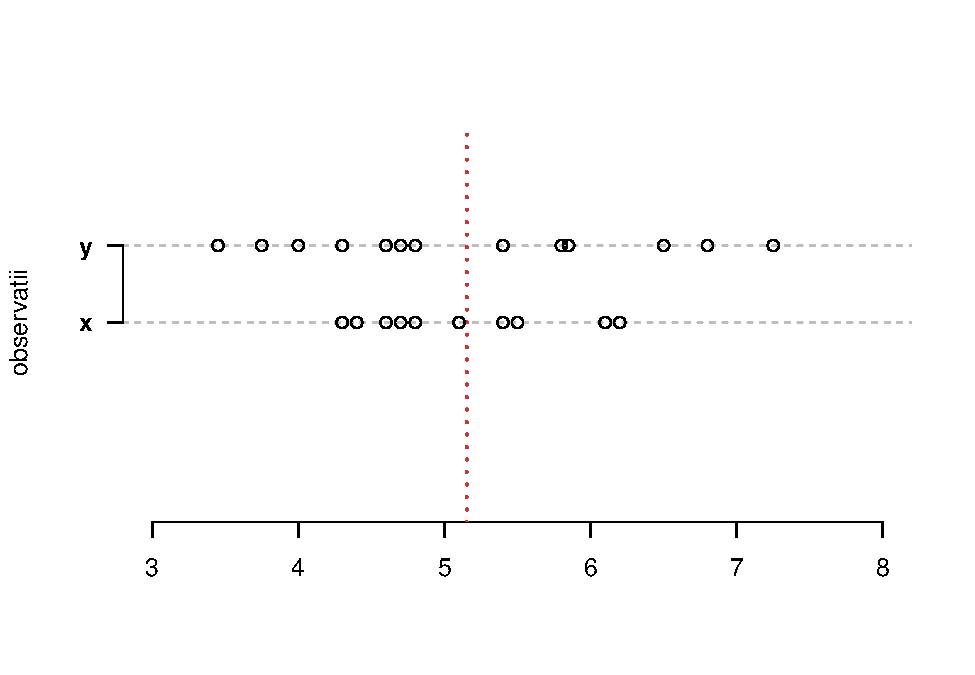
\includegraphics[width=0.8\linewidth]{Lab_2_files/figure-latex/unnamed-chunk-12-1} \end{center}

\subsection{Varianța și abaterea
standard}\label{varianta-si-abaterea-standard}

Varianța eșantionului se calculează cu ajutorul formulei

\[
  S_n^2 = \frac{1}{n-1}\sum_{i=1}^{n}\left(X_i - \bar{X}_n\right)^2
\]

iar abaterea standard a eșantionului este \(s_d = \sqrt{S_n^2}\)
(măsurată în aceleași unități de măsură ca și datele inițiale).

\begin{Shaded}
\begin{Highlighting}[]
\CommentTok{# varianta }
\KeywordTok{var}\NormalTok{(chickwts}\OperatorTok{$}\NormalTok{weight[chickwts}\OperatorTok{$}\NormalTok{feed }\OperatorTok{==}\StringTok{ "soybean"}\NormalTok{])}
\NormalTok{[}\DecValTok{1}\NormalTok{] }\FloatTok{2929.956}

\CommentTok{# abaterea standard}
\KeywordTok{sd}\NormalTok{(chickwts}\OperatorTok{$}\NormalTok{weight[chickwts}\OperatorTok{$}\NormalTok{feed }\OperatorTok{==}\StringTok{ "soybean"}\NormalTok{])}
\NormalTok{[}\DecValTok{1}\NormalTok{] }\FloatTok{54.12907}
\end{Highlighting}
\end{Shaded}

\subsection{Intervalul dintre
cuartile}\label{intervalul-dintre-cuartile}

Intervalul dintre cuartile măsoară distanța dintre a treia cuartilă și
prima curtilă

\[
  IQR = Q_3 - Q_1
\] precizând care este lungimea intervalului pe care se regăsesc
aproximativ jumătate dintre obserevații (observațiile de mijloc).

\begin{Shaded}
\begin{Highlighting}[]
\KeywordTok{IQR}\NormalTok{(chickwts}\OperatorTok{$}\NormalTok{weight)}
\NormalTok{[}\DecValTok{1}\NormalTok{] }\DecValTok{119}
\KeywordTok{IQR}\NormalTok{(chickwts}\OperatorTok{$}\NormalTok{weight[chickwts}\OperatorTok{$}\NormalTok{feed }\OperatorTok{==}\StringTok{ "horsebean"}\NormalTok{])}
\NormalTok{[}\DecValTok{1}\NormalTok{] }\FloatTok{39.25}
\end{Highlighting}
\end{Shaded}

\section{Metode grafice}\label{metode-grafice}

\subsection{Diagrama cu bare (barplot)}\label{diagrama-cu-bare-barplot}

Diagrama cu batoane sau bare (\emph{barplot}) este o metodă grafică
folosită cu precădere atunci când datele sunt calitative (sau discrete).
O diagramă de tip barplot trasează bare verticale sau orizontale, în
general separate de un spațiu alb, pentru a evidenția frecevențele de
apariție a observațiilor după categoriile corespunzătoare.

Să presupunem că \(X\) este o variabilă aleatoare discretă cu funcția de
masă dată de \(p(x)=\mathbb{P}(X = x)\) și \(X_1, X_2, \ldots, X_n\) un
eșantion de talie \(n\) din populația \(p(x)\). Dacă \(X\) ia un număr
finit de valori, \(X\in\mathcal{A}\) cu
\(\mathcal{A} = \{a_1, \ldots, a_m\}\), atunci un estimator al lui
\(p(a_j)\) este

\[
  \hat{p}(a_j) = \frac{1}{n}\sum_{i = 1}^{n}\mathbf{1}_{\left\{X_i = a_j\right\}}.
\]

Dacă \(X\) ia un număr infinit de valori, \(X\in\mathcal{A}\) cu
\(\mathcal{A} = \{a_1, a_2, \ldots\}\), atunci formăm grupurile

\[
  \{a_1\}, \;\{a_2\},\cdots, \{a_m\},\; \tilde{a}_{m+1} = \{a_{m+1}, a_{m+2}, \ldots\}
\]

și considerăm

\[
  \hat{p}(\tilde{a}_{m+1}) = \frac{1}{n}\sum_{i = 1}^{n}\mathbf{1}_{\left\{X_i \geq a_{m+1}\right\}}.
\] În practică, alegerea lui \(m\) se face așa încât
\(\hat{p}(a_m)\geq 2\hat{p}(\tilde{a}_{m+1})\). O diagramă cu bare este
o ilustrare a lui \(a_j\) versus \(\hat{p}(a_j)\).

În R se folosește funcția \texttt{barplot()}:

\begin{Shaded}
\begin{Highlighting}[]
\KeywordTok{barplot}\NormalTok{(}\KeywordTok{table}\NormalTok{(chickwts}\OperatorTok{$}\NormalTok{feed))}
\end{Highlighting}
\end{Shaded}

\begin{center}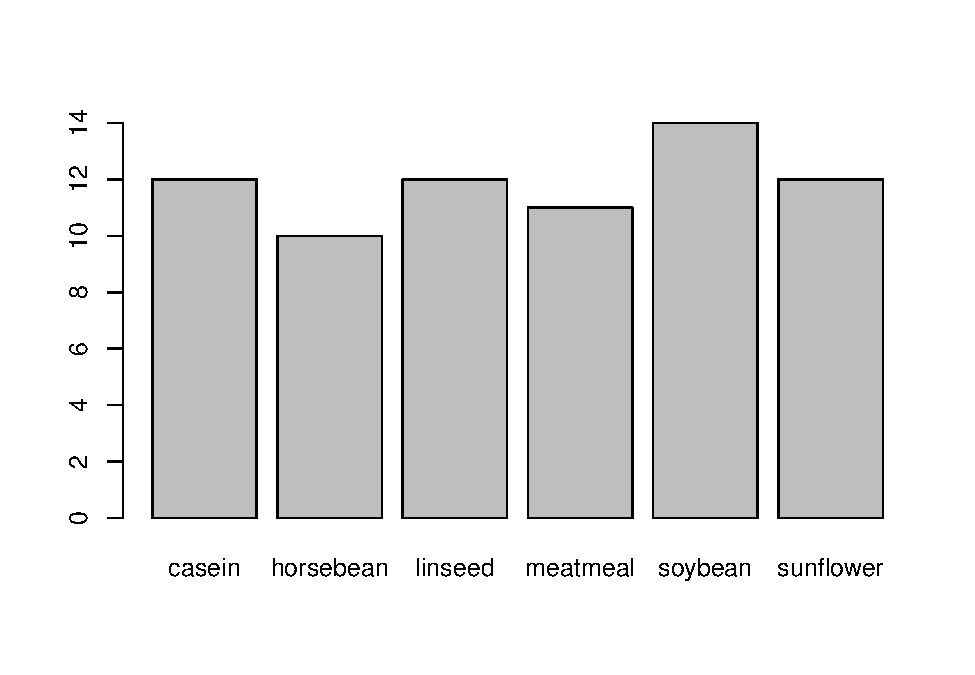
\includegraphics[width=0.7\linewidth]{Lab_2_files/figure-latex/unnamed-chunk-15-1} \end{center}

Setul de date \texttt{birthwt} din pachetul \texttt{MASS} este descris
de:

\begin{longtable}[]{@{}ll@{}}
\toprule
Variabila & Scurtă descriere\tabularnewline
\midrule
\endhead
low & indică dacă greutatea la naștere este mai mică decât
2.5Kg\tabularnewline
age & vârsta mamei în ani\tabularnewline
lwt & greutatea mamei înainet de naștere\tabularnewline
rage & rasa mamei (1 = alb, 2 = negru, 3 = altele)\tabularnewline
smoke & statutul de fumător al mamei pe parcursul
sarcinii\tabularnewline
ptl & numărul de sarcini premature anterioare\tabularnewline
ht & istoricul de hipertensiune a mamei\tabularnewline
ui & prezența iretabilității uterine\tabularnewline
ftv & numărul de vizite la doctor din primul trimestru de
sarcină\tabularnewline
bwt & greutatea la naștere a copilului în grame\tabularnewline
\bottomrule
\end{longtable}

\begin{Shaded}
\begin{Highlighting}[]
\KeywordTok{library}\NormalTok{(MASS)}
\KeywordTok{head}\NormalTok{(birthwt)}
\NormalTok{   low age lwt race smoke ptl ht ui ftv  bwt}
\DecValTok{85}   \DecValTok{0}  \DecValTok{19} \DecValTok{182}    \DecValTok{2}     \DecValTok{0}   \DecValTok{0}  \DecValTok{0}  \DecValTok{1}   \DecValTok{0} \DecValTok{2523}
\DecValTok{86}   \DecValTok{0}  \DecValTok{33} \DecValTok{155}    \DecValTok{3}     \DecValTok{0}   \DecValTok{0}  \DecValTok{0}  \DecValTok{0}   \DecValTok{3} \DecValTok{2551}
\DecValTok{87}   \DecValTok{0}  \DecValTok{20} \DecValTok{105}    \DecValTok{1}     \DecValTok{1}   \DecValTok{0}  \DecValTok{0}  \DecValTok{0}   \DecValTok{1} \DecValTok{2557}
\DecValTok{88}   \DecValTok{0}  \DecValTok{21} \DecValTok{108}    \DecValTok{1}     \DecValTok{1}   \DecValTok{0}  \DecValTok{0}  \DecValTok{1}   \DecValTok{2} \DecValTok{2594}
\DecValTok{89}   \DecValTok{0}  \DecValTok{18} \DecValTok{107}    \DecValTok{1}     \DecValTok{1}   \DecValTok{0}  \DecValTok{0}  \DecValTok{1}   \DecValTok{0} \DecValTok{2600}
\DecValTok{91}   \DecValTok{0}  \DecValTok{21} \DecValTok{124}    \DecValTok{3}     \DecValTok{0}   \DecValTok{0}  \DecValTok{0}  \DecValTok{0}   \DecValTok{0} \DecValTok{2622}
\end{Highlighting}
\end{Shaded}

Ne propunem să ilustrăm distribuția greutății la naștere a copiilor după
categoriile: ``\textless{}1500'', ``1500-2000'', ``2000-2500'',
``2500-3000'', ``3000-3500'', ``3500+''.

\begin{Shaded}
\begin{Highlighting}[]
\NormalTok{dat.birthwt =}\StringTok{ }\NormalTok{birthwt }
\NormalTok{dat.birthwt}\OperatorTok{$}\NormalTok{wtcut =}\StringTok{ }\KeywordTok{cut}\NormalTok{(dat.birthwt}\OperatorTok{$}\NormalTok{bwt, }
                        \DataTypeTok{breaks =} \KeywordTok{c}\NormalTok{(}\DecValTok{0}\NormalTok{, }\DecValTok{1500}\NormalTok{, }\DecValTok{2000}\NormalTok{, }\DecValTok{2500}\NormalTok{, }\DecValTok{3000}\NormalTok{, }\DecValTok{3500}\NormalTok{, }
                                   \KeywordTok{max}\NormalTok{(dat.birthwt}\OperatorTok{$}\NormalTok{bwt)),}
                        \DataTypeTok{labels =} \KeywordTok{c}\NormalTok{(}\StringTok{"<1500"}\NormalTok{, }\StringTok{"1500-2000"}\NormalTok{, }
                                   \StringTok{"2000-2500"}\NormalTok{, }\StringTok{"2500-3000"}\NormalTok{,}
                                   \StringTok{"3000-3500"}\NormalTok{, }\StringTok{"3500+"}\NormalTok{))}

\KeywordTok{barplot}\NormalTok{(}\KeywordTok{table}\NormalTok{(dat.birthwt}\OperatorTok{$}\NormalTok{wtcut),}
        \DataTypeTok{cex.names =} \FloatTok{0.7}\NormalTok{)}
\end{Highlighting}
\end{Shaded}

\begin{center}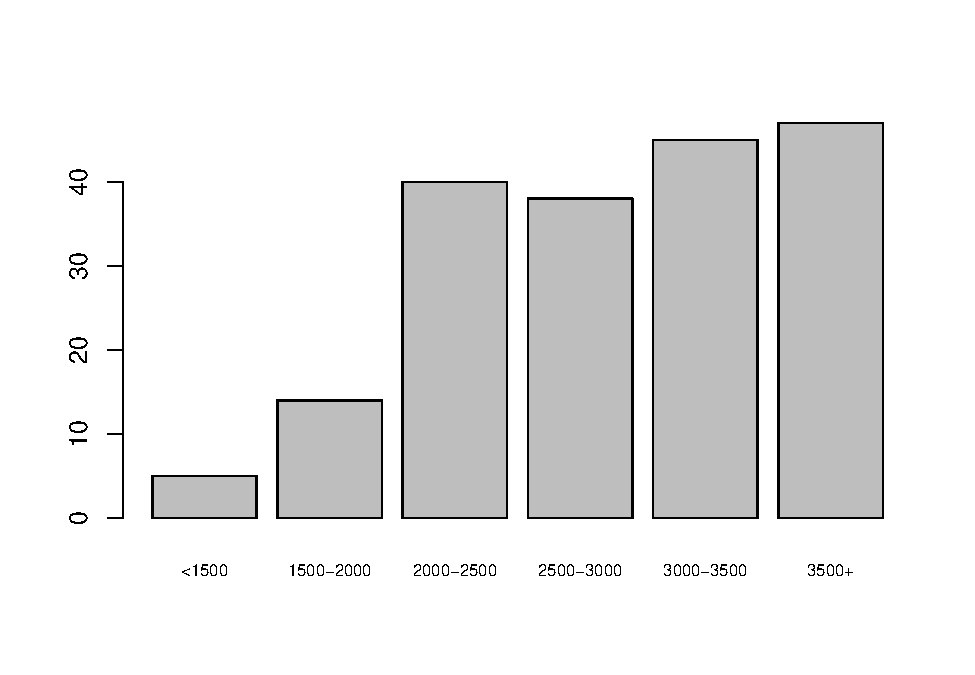
\includegraphics[width=0.7\linewidth]{Lab_2_files/figure-latex/unnamed-chunk-17-1} \end{center}

și în funcție de statutul de fumător al mamei

\begin{Shaded}
\begin{Highlighting}[]
\KeywordTok{barplot}\NormalTok{(}\KeywordTok{table}\NormalTok{(dat.birthwt}\OperatorTok{$}\NormalTok{smoke, dat.birthwt}\OperatorTok{$}\NormalTok{wtcut),}
        \DataTypeTok{beside =} \OtherTok{TRUE}\NormalTok{, }
        \DataTypeTok{horiz =} \OtherTok{TRUE}\NormalTok{, }\DataTypeTok{las =} \DecValTok{1}\NormalTok{,}
        \DataTypeTok{main =} \StringTok{"Greutatea la nastere in functie de }\CharTok{\textbackslash{}n}\StringTok{statutul de fumator al mamei"}\NormalTok{,}
        \DataTypeTok{legend.text=}\KeywordTok{c}\NormalTok{(}\StringTok{"nefumator"}\NormalTok{,}\StringTok{"fumator"}\NormalTok{),}
        \DataTypeTok{args.legend=}\KeywordTok{list}\NormalTok{(}\DataTypeTok{x=}\StringTok{"bottomright"}\NormalTok{, }\DataTypeTok{bty =} \StringTok{"n"}\NormalTok{),}
        \DataTypeTok{cex.names =} \FloatTok{0.7}\NormalTok{)}
\end{Highlighting}
\end{Shaded}

\begin{center}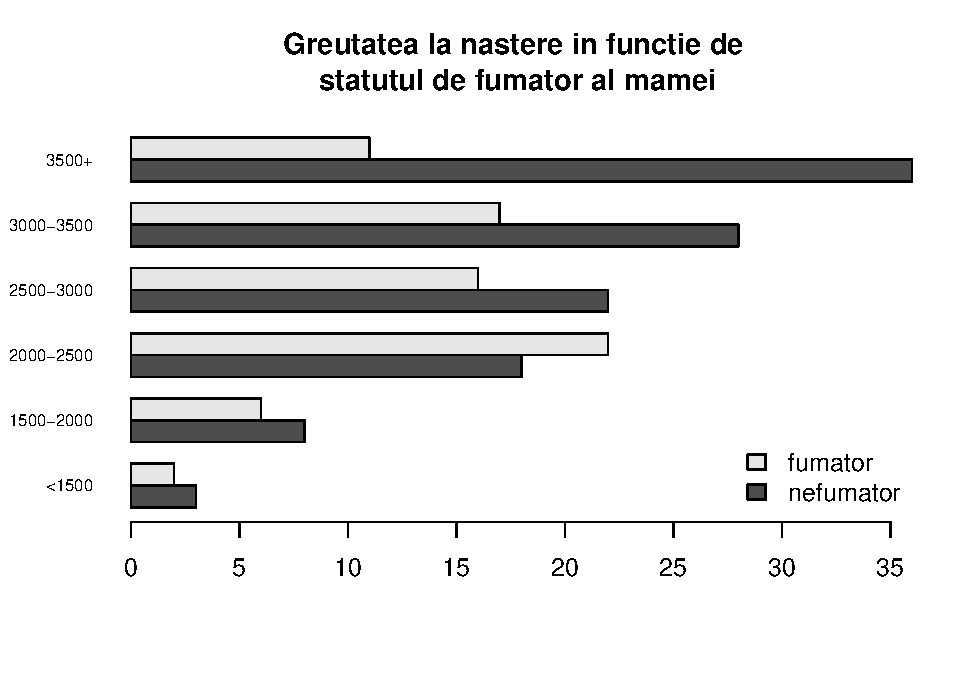
\includegraphics[width=0.7\linewidth]{Lab_2_files/figure-latex/unnamed-chunk-18-1} \end{center}

\subsection{Histograma}\label{histograma}

\emph{Histograma} este un exemplu de metodă neparametrică de estimare a
densității de probabilitate. Fie \(X_1, X_2, \ldots, X_n\) un eșantion
de talie \(n\) dintr-o populație cu densitate de probabilitate \(f\).
Fără a restrânge generalitatea putem să presupunem că \(X_i\in[0,1]\)
(în caz contrar putem scala observațiile la acest interval).

Fie \(m\) un număr natural și să considerăm diviziunea intervalului
\([0,1]\) (fiecare subinterval din diviziune se numește \emph{bin}):

\[
  B_1 = \left[0, \frac{1}{m}\right), \, B_2 = \left[\frac{1}{m}, \frac{2}{m}\right),\cdots,\, B_m = \left[\frac{m-1}{m}, 1\right].
\]

Notăm cu \(h = \frac{1}{m}\) lungimea bin-urilor,
\(p_j = \mathbb{P}(X_i\in B_j) = \int_{B_j}f(t)\,dt\) probabilitatea ca
o observație să pice în subintervalul \(B_j\) și
\(\hat{p}_j = \frac{1}{n}\sum_{i = 1}^{n}\mathbf{1}_{\left\{X_i \in B_j\right\}}\)
numărul de observații, din cele \(n\), care se află în intervalul
\(B_j\). Atunci estimatorul \emph{histogramă} este dat de

\[
  \hat{f}_n(x) = \left\{\begin{array}{llll}
            \frac{\hat{p}_1}{h}, & x\in B_1\\
            \frac{\hat{p}_2}{h}, & x\in B_2\\
            \vdots, & \vdots\\
            \frac{\hat{p}_m}{h}, & x\in B_m
  \end{array}\right.
\]

care scris sub formă compactă devine

\[
  \hat{f}_n(x) = \sum_{i=1}^{m} \frac{\hat{p}_i}{h} \mathbf{1}_{B_i}(x).
\] Se poate observa că pentru \(m\) suficient de mare (\(h\) mic) și
\(x\in B_j\) avem

\[
  \mathbb{E}\left[\hat{f}_n(x)\right] = \mathbb{E}\left[\sum_{i=1}^{m} \frac{\hat{p}_i}{h} \mathbf{1}_{B_i}(x)\right]= \frac{\mathbb{E}\left[\hat{p}_j\right]}{h} = \frac{p_j}{h} = \frac{\int_{B_j}f(x)\,dx}{h}\approx \frac{f(x)h}{h} = f(x).
\] Alegerea numărului de bin-uri și a mărimii acestora nu este o
problemă trivială. De exemplu, D. Scott propune o variantă de alegere a
lui \(k\) în articolul (Scott 1979). Un rezultat similar, dar mai
robust, a fost obținut de D. Freedman și P. Diaconis în (Freedman and
Diaconis 1981). Câteva dintre metodele de alegere a mărimii bin-ului
sunt prezentate în următoarea pagină de
\href{https://en.wikipedia.org/wiki/Histogram\#Number_of_bins_and_width}{Wikipedia}.

În R, funcția \texttt{hist()} este folosită pentru trasarea unei
histograme. Această funcție utilizează ca metodă predefinită de alegere
a mărimii bin-urilor, metoda lui Sturges (a se vedea articolul (Sturges
1926)).

\begin{rmdexercise}
Considerați setul de date \texttt{chickwts}. Investigați cu ajutorul
unei histograme cum este repartizată greutatea găinilor, variabila
\texttt{weight}. Dar în funcție de tipul de alimentație \texttt{feed} ?.
\end{rmdexercise}

\begin{Shaded}
\begin{Highlighting}[]
\KeywordTok{par}\NormalTok{(}\DataTypeTok{mfrow =} \KeywordTok{c}\NormalTok{(}\DecValTok{1}\NormalTok{,}\DecValTok{3}\NormalTok{))}

\KeywordTok{hist}\NormalTok{(chickwts}\OperatorTok{$}\NormalTok{weight, }
     \DataTypeTok{probability =} \OtherTok{TRUE}\NormalTok{, }
     \DataTypeTok{col =} \StringTok{"grey80"}\NormalTok{,}
     \DataTypeTok{main =} \StringTok{"Repartitia greutatii}\CharTok{\textbackslash{}n}\StringTok{ (Sturges)"}\NormalTok{,}
     \DataTypeTok{xlab =} \StringTok{""}\NormalTok{,}
     \DataTypeTok{ylab =} \StringTok{"Densitatea"}\NormalTok{)}

\KeywordTok{hist}\NormalTok{(chickwts}\OperatorTok{$}\NormalTok{weight, }
     \DataTypeTok{probability =} \OtherTok{TRUE}\NormalTok{, }
     \DataTypeTok{breaks =} \StringTok{"FD"}\NormalTok{,}
     \DataTypeTok{col =} \StringTok{"grey80"}\NormalTok{,}
     \DataTypeTok{main =} \StringTok{"Repartitia greutatii}\CharTok{\textbackslash{}n}\StringTok{ (Freedman-Diaconis)"}\NormalTok{,}
     \DataTypeTok{xlab =} \StringTok{""}\NormalTok{,}
     \DataTypeTok{ylab =} \StringTok{"Densitatea"}\NormalTok{)}

\KeywordTok{hist}\NormalTok{(chickwts}\OperatorTok{$}\NormalTok{weight, }
     \DataTypeTok{probability =} \OtherTok{TRUE}\NormalTok{, }
     \DataTypeTok{breaks =} \KeywordTok{seq}\NormalTok{(}\DecValTok{100}\NormalTok{, }\DecValTok{450}\NormalTok{, }\DecValTok{25}\NormalTok{),}
     \DataTypeTok{col =} \StringTok{"grey80"}\NormalTok{,}
     \DataTypeTok{main =} \StringTok{"Repartitia greutatii}\CharTok{\textbackslash{}n}\StringTok{ (marimea bin-ului 25)"}\NormalTok{,}
     \DataTypeTok{xlab =} \StringTok{""}\NormalTok{,}
     \DataTypeTok{ylab =} \StringTok{"Densitatea"}\NormalTok{)}
\end{Highlighting}
\end{Shaded}

\begin{center}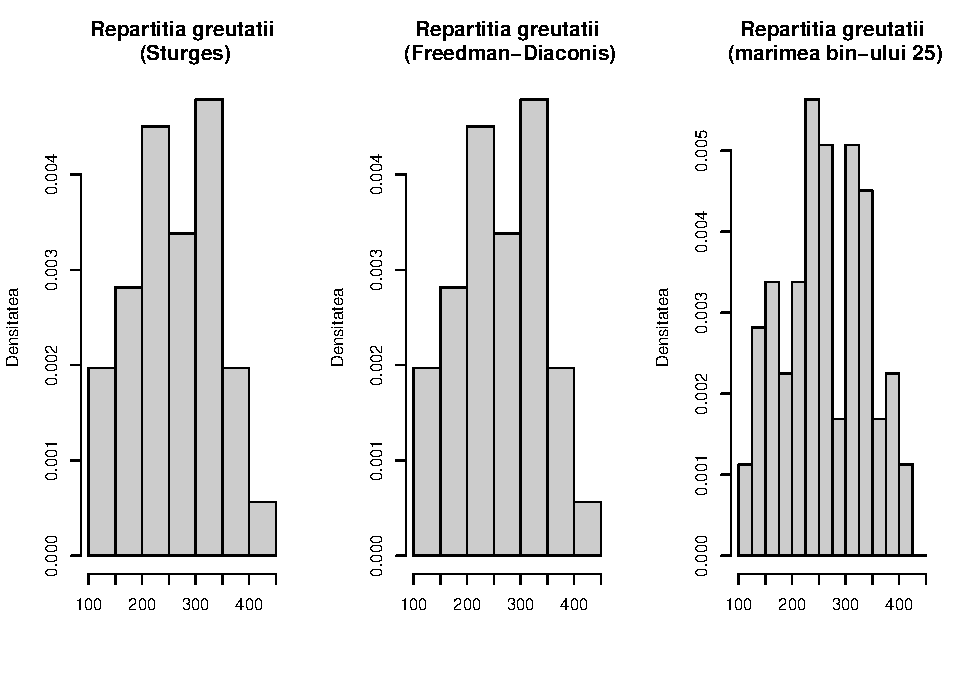
\includegraphics[width=0.7\linewidth]{Lab_2_files/figure-latex/unnamed-chunk-20-1} \end{center}

\begin{rmdexercise}
Considerați setul de date \texttt{mtcars}. Investigați cu ajutorul unei
histograme cum este repartizată variabila \texttt{hp}. Trasați prin
drepte verticale de culori diferite media și respectiv mediana datelor.
\end{rmdexercise}

\begin{Shaded}
\begin{Highlighting}[]
\KeywordTok{par}\NormalTok{(}\DataTypeTok{mfrow =} \KeywordTok{c}\NormalTok{(}\DecValTok{1}\NormalTok{,}\DecValTok{2}\NormalTok{))}

\KeywordTok{hist}\NormalTok{(mtcars}\OperatorTok{$}\NormalTok{hp, }\DataTypeTok{freq =} \OtherTok{FALSE}\NormalTok{,}
     \DataTypeTok{main =} \StringTok{"Horepower - HP}\CharTok{\textbackslash{}n}\StringTok{ (default)"}\NormalTok{, }
     \DataTypeTok{xlab=}\StringTok{"HP"}\NormalTok{)}

\KeywordTok{hist}\NormalTok{(mtcars}\OperatorTok{$}\NormalTok{hp, }\DataTypeTok{freq =} \OtherTok{FALSE}\NormalTok{,}
     \DataTypeTok{breaks=}\KeywordTok{seq}\NormalTok{(}\DecValTok{0}\NormalTok{,}\DecValTok{400}\NormalTok{,}\DecValTok{25}\NormalTok{),}
     \DataTypeTok{col=}\StringTok{"gray"}\NormalTok{,}
     \DataTypeTok{main=}\StringTok{"Horsepower - HP}\CharTok{\textbackslash{}n}\StringTok{ (marimea bin-ului 25)"}\NormalTok{,}
     \DataTypeTok{xlab=}\StringTok{"HP"}\NormalTok{)}

\KeywordTok{abline}\NormalTok{(}\DataTypeTok{v=}\KeywordTok{c}\NormalTok{(}\KeywordTok{mean}\NormalTok{(mtcars}\OperatorTok{$}\NormalTok{hp), }\KeywordTok{median}\NormalTok{(mtcars}\OperatorTok{$}\NormalTok{hp)), }
       \DataTypeTok{lty=}\KeywordTok{c}\NormalTok{(}\DecValTok{2}\NormalTok{,}\DecValTok{3}\NormalTok{), }\DataTypeTok{lwd=}\DecValTok{2}\NormalTok{)}
\KeywordTok{legend}\NormalTok{(}\StringTok{"topright"}\NormalTok{, }\DataTypeTok{legend=}\KeywordTok{c}\NormalTok{(}\StringTok{"media HP"}\NormalTok{,}\StringTok{"mediana HP"}\NormalTok{),}
       \DataTypeTok{lty=}\KeywordTok{c}\NormalTok{(}\DecValTok{2}\NormalTok{,}\DecValTok{3}\NormalTok{), }\DataTypeTok{lwd=}\DecValTok{2}\NormalTok{,}
       \DataTypeTok{bty =} \StringTok{"n"}\NormalTok{)}
\end{Highlighting}
\end{Shaded}

\begin{center}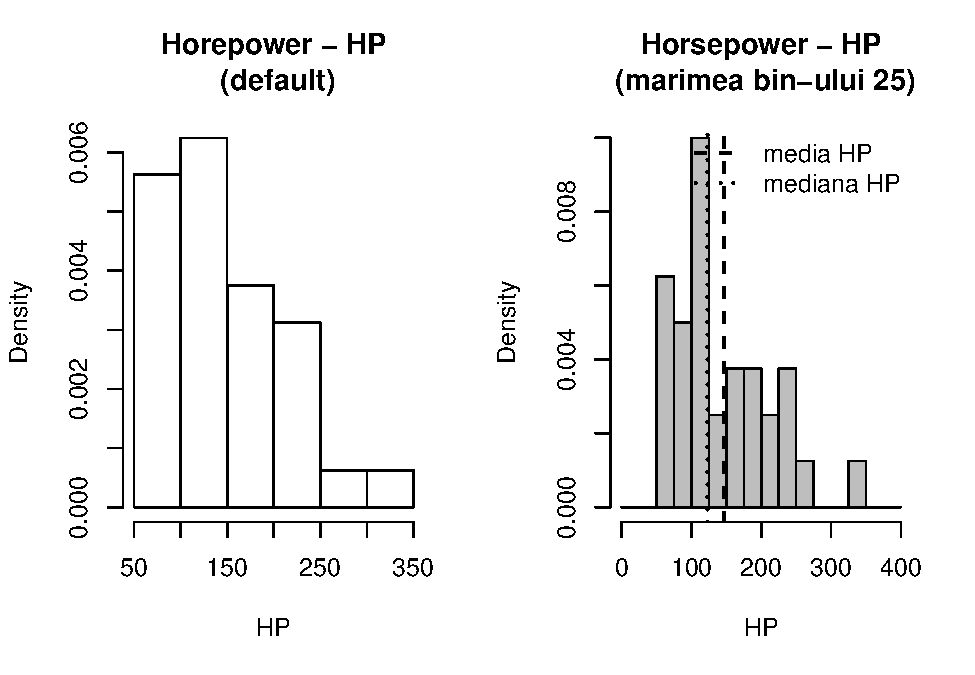
\includegraphics[width=0.7\linewidth]{Lab_2_files/figure-latex/unnamed-chunk-22-1} \end{center}

\begin{rmdexercise}
Să presupunem că în fișierul
\href{\%22dataIn/studFMI.txt\%22}{studFMI.txt} am stocat date privind
sexul (f/h), înălțimea (în cm) și greutatea (în kg) a studenților de
master de la Facultatea de Matematică și Informatică. Vrem să
investigăm, trasând pe același grafic, cum este repartizată înălțimea și
respectiv greutatea studenților în funcție de sex.
\end{rmdexercise}

Începem prin a citi datele din fișier:

\begin{Shaded}
\begin{Highlighting}[]
\NormalTok{stud =}\StringTok{ }\KeywordTok{read.table}\NormalTok{(}\StringTok{"dataIn/studFMI.txt"}\NormalTok{, }\DataTypeTok{header =} \OtherTok{TRUE}\NormalTok{)}
\KeywordTok{str}\NormalTok{(stud)}
\StringTok{'data.frame'}\OperatorTok{:}\StringTok{   }\DecValTok{97}\NormalTok{ obs. of  }\DecValTok{3}\NormalTok{ variables}\OperatorTok{:}
\StringTok{ }\ErrorTok{$}\StringTok{ }\NormalTok{sex   }\OperatorTok{:}\StringTok{ }\NormalTok{Factor w}\OperatorTok{/}\StringTok{ }\DecValTok{2}\NormalTok{ levels }\StringTok{"f"}\NormalTok{,}\StringTok{"h"}\OperatorTok{:}\StringTok{ }\DecValTok{2} \DecValTok{2} \DecValTok{1} \DecValTok{1} \DecValTok{2} \DecValTok{1} \DecValTok{2} \DecValTok{2} \DecValTok{2} \DecValTok{2}\NormalTok{ ...}
 \OperatorTok{$}\StringTok{ }\NormalTok{height}\OperatorTok{:}\StringTok{ }\NormalTok{int  }\DecValTok{168} \DecValTok{177} \DecValTok{164} \DecValTok{166} \DecValTok{165} \DecValTok{150} \DecValTok{186} \DecValTok{185} \DecValTok{181} \DecValTok{188}\NormalTok{ ...}
 \OperatorTok{$}\StringTok{ }\NormalTok{weight}\OperatorTok{:}\StringTok{ }\NormalTok{int  }\DecValTok{69} \DecValTok{73} \DecValTok{53} \DecValTok{57} \DecValTok{60} \DecValTok{42} \DecValTok{74} \DecValTok{83} \DecValTok{77} \DecValTok{72}\NormalTok{ ...}
\KeywordTok{head}\NormalTok{(stud)}
\NormalTok{  sex height weight}
\DecValTok{1}\NormalTok{   h    }\DecValTok{168}     \DecValTok{69}
\DecValTok{2}\NormalTok{   h    }\DecValTok{177}     \DecValTok{73}
\DecValTok{3}\NormalTok{   f    }\DecValTok{164}     \DecValTok{53}
\DecValTok{4}\NormalTok{   f    }\DecValTok{166}     \DecValTok{57}
\DecValTok{5}\NormalTok{   h    }\DecValTok{165}     \DecValTok{60}
\DecValTok{6}\NormalTok{   f    }\DecValTok{150}     \DecValTok{42}
\end{Highlighting}
\end{Shaded}

Separăm înălțimea (greutatea este exercițiu!) bărbaților și a femeilor:

\begin{Shaded}
\begin{Highlighting}[]
\CommentTok{# h vine de la hommes iar f de la femmes}
\NormalTok{hm =}\StringTok{ }\NormalTok{stud}\OperatorTok{$}\NormalTok{height[stud}\OperatorTok{$}\NormalTok{sex }\OperatorTok{==}\StringTok{ "h"}\NormalTok{]}
\NormalTok{hf =}\StringTok{ }\NormalTok{stud}\OperatorTok{$}\NormalTok{height[stud}\OperatorTok{$}\NormalTok{sex }\OperatorTok{==}\StringTok{ "f"}\NormalTok{]}

\KeywordTok{par}\NormalTok{(}\DataTypeTok{mfrow =} \KeywordTok{c}\NormalTok{(}\DecValTok{1}\NormalTok{,}\DecValTok{2}\NormalTok{))}

\KeywordTok{hist}\NormalTok{(hm, }\DataTypeTok{freq =} \OtherTok{FALSE}\NormalTok{, }\DataTypeTok{col =} \KeywordTok{grey}\NormalTok{(}\FloatTok{0.8}\NormalTok{),}
     \DataTypeTok{main =} \StringTok{"Inaltimea barbatilor"}\NormalTok{, }
     \DataTypeTok{xlab =} \StringTok{"inaltimea"}\NormalTok{,}
     \DataTypeTok{ylab =} \StringTok{"densitatea"}\NormalTok{)}
\NormalTok{tm =}\StringTok{ }\KeywordTok{seq}\NormalTok{(}\KeywordTok{min}\NormalTok{(hm)}\OperatorTok{-}\DecValTok{5}\NormalTok{, }\KeywordTok{max}\NormalTok{(hm)}\OperatorTok{+}\DecValTok{5}\NormalTok{, }\DataTypeTok{length.out =} \DecValTok{100}\NormalTok{)}
\KeywordTok{lines}\NormalTok{(tm, }\KeywordTok{dnorm}\NormalTok{(tm, }\KeywordTok{mean}\NormalTok{(hm), }\KeywordTok{sd}\NormalTok{(hm)), }
      \DataTypeTok{lty =} \DecValTok{2}\NormalTok{, }\DataTypeTok{lwd =} \DecValTok{2}\NormalTok{)}

\KeywordTok{hist}\NormalTok{(hf, }\DataTypeTok{freq =} \OtherTok{FALSE}\NormalTok{, }\DataTypeTok{col =} \KeywordTok{grey}\NormalTok{(}\FloatTok{0.8}\NormalTok{),}
     \DataTypeTok{main =} \StringTok{"Inaltimea femeilor"}\NormalTok{, }
     \DataTypeTok{xlab =} \StringTok{"inaltimea"}\NormalTok{,}
     \DataTypeTok{ylab =} \StringTok{"densitatea"}\NormalTok{)}
\NormalTok{tf =}\StringTok{ }\KeywordTok{seq}\NormalTok{(}\KeywordTok{min}\NormalTok{(hf)}\OperatorTok{-}\DecValTok{5}\NormalTok{, }\KeywordTok{max}\NormalTok{(hf)}\OperatorTok{+}\DecValTok{5}\NormalTok{, }\DataTypeTok{length.out =} \DecValTok{100}\NormalTok{)}
\KeywordTok{lines}\NormalTok{(tf, }\KeywordTok{dnorm}\NormalTok{(tf, }\KeywordTok{mean}\NormalTok{(hf), }\KeywordTok{sd}\NormalTok{(hf)), }
      \DataTypeTok{lty =} \DecValTok{2}\NormalTok{, }\DataTypeTok{lwd =} \DecValTok{2}\NormalTok{)}
\end{Highlighting}
\end{Shaded}

\begin{center}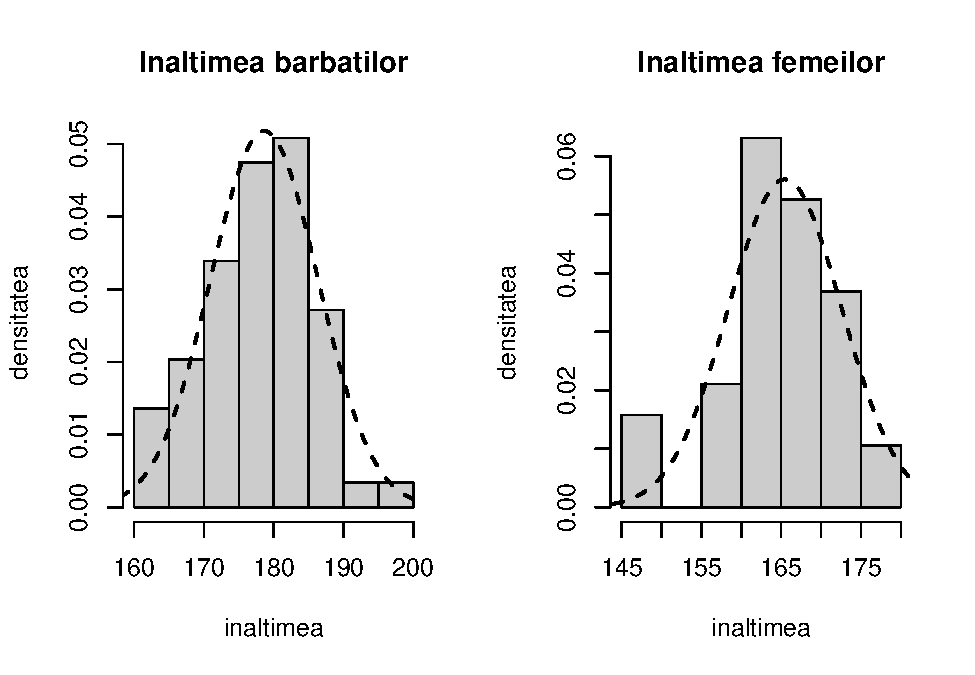
\includegraphics[width=0.8\linewidth]{Lab_2_files/figure-latex/unnamed-chunk-25-1} \end{center}

Reprezentăm repartiția înălțimilor luate împreună și evidențiem mixtura
celor două repartiții după sex:

\begin{Shaded}
\begin{Highlighting}[]
\NormalTok{height =}\StringTok{ }\NormalTok{stud}\OperatorTok{$}\NormalTok{height}

\KeywordTok{hist}\NormalTok{(height, }\DataTypeTok{proba =} \OtherTok{TRUE}\NormalTok{, }
     \DataTypeTok{breaks=}\DecValTok{25}\NormalTok{, }
     \DataTypeTok{col =} \KeywordTok{grey}\NormalTok{(}\FloatTok{0.8}\NormalTok{), }
     \DataTypeTok{main =} \StringTok{"Inaltimea barbatilor si a femeilor"}\NormalTok{,}
     \DataTypeTok{xlab =} \StringTok{"inaltimea"}\NormalTok{,}
     \DataTypeTok{ylab =} \StringTok{"densitatea"}\NormalTok{,}
     \DataTypeTok{ylim =} \KeywordTok{c}\NormalTok{(}\DecValTok{0}\NormalTok{, }\FloatTok{0.05}\NormalTok{))}

\NormalTok{t <-}\StringTok{ }\KeywordTok{seq}\NormalTok{(}\DecValTok{145}\NormalTok{,}\DecValTok{200}\NormalTok{,}\DataTypeTok{length=}\DecValTok{100}\NormalTok{)}

\NormalTok{x1 <-}\StringTok{ }\KeywordTok{dnorm}\NormalTok{(t,}\KeywordTok{mean}\NormalTok{(hf),}\KeywordTok{sd}\NormalTok{(hf))}
\NormalTok{x2 <-}\StringTok{ }\KeywordTok{dnorm}\NormalTok{(t,}\KeywordTok{mean}\NormalTok{(hm),}\KeywordTok{sd}\NormalTok{(hm))}

\CommentTok{# proportia de femei (din nr de studenti)}
\NormalTok{pf <-}\StringTok{ }\KeywordTok{length}\NormalTok{(hf)}\OperatorTok{/}\KeywordTok{length}\NormalTok{(height)}

\CommentTok{# mixtura dintre rep inaltimilor f si h}
\NormalTok{x3 <-}\StringTok{ }\NormalTok{pf}\OperatorTok{*}\NormalTok{x1 }\OperatorTok{+}\StringTok{ }\NormalTok{(}\DecValTok{1}\OperatorTok{-}\NormalTok{pf)}\OperatorTok{*}\NormalTok{x2}

\KeywordTok{lines}\NormalTok{(t, x3, }\DataTypeTok{lwd =} \DecValTok{2}\NormalTok{)}

\KeywordTok{lines}\NormalTok{(t, pf}\OperatorTok{*}\NormalTok{x1, }\DataTypeTok{col =} \StringTok{"brown3"}\NormalTok{, }
      \DataTypeTok{lty =} \DecValTok{2}\NormalTok{, }\DataTypeTok{lwd =} \DecValTok{2}\NormalTok{)}
\KeywordTok{lines}\NormalTok{(t, (}\DecValTok{1}\OperatorTok{-}\NormalTok{pf)}\OperatorTok{*}\NormalTok{x2, }\DataTypeTok{col =} \StringTok{"royalblue"}\NormalTok{, }
      \DataTypeTok{lty =} \DecValTok{2}\NormalTok{, }\DataTypeTok{lwd =} \DecValTok{2}\NormalTok{)}

\KeywordTok{legend}\NormalTok{(}\StringTok{"topright"}\NormalTok{, }\KeywordTok{c}\NormalTok{(}\StringTok{"femei"}\NormalTok{,}\StringTok{"barbati"}\NormalTok{), }
       \DataTypeTok{col =} \KeywordTok{c}\NormalTok{(}\StringTok{"brown3"}\NormalTok{,}\StringTok{"royalblue"}\NormalTok{), }
       \DataTypeTok{lty =} \DecValTok{2}\NormalTok{, }\DataTypeTok{lwd =} \DecValTok{2}\NormalTok{, }
       \DataTypeTok{bty =} \StringTok{"n"}\NormalTok{)}
\end{Highlighting}
\end{Shaded}

\begin{center}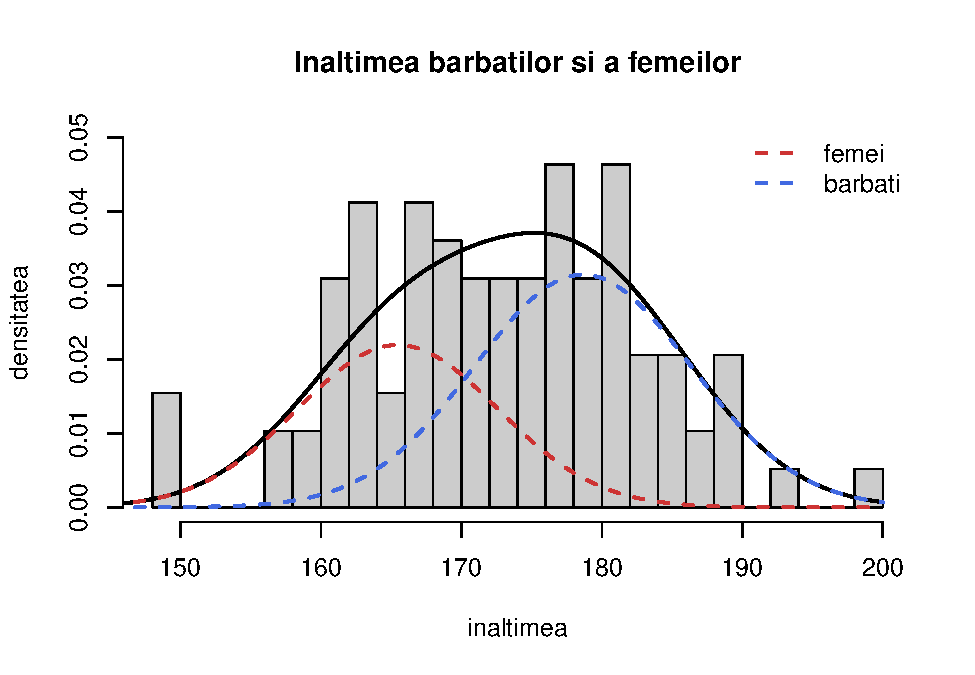
\includegraphics[width=0.8\linewidth]{Lab_2_files/figure-latex/unnamed-chunk-26-1} \end{center}

\subsection{Boxplot}\label{boxplot}

Una dintre metodele grafice des întâlnite în vizualizarea datelor
(cantitative) unidimensionale este \emph{boxplot}-ul (eng. \emph{box and
whisker plot} - cutia cu mustăți). Această metodă grafică descriptivă
este folosită în principal pentru a investiga forma repartiției
(simetrică sau asimetrică) datelor dar și variabilitatea acestora precum
și pentru detectarea și ilustrarea schimbărilor de locație și variație
între diferitele grupuri de date.

După cum putem vedea și în figura de mai jos, cutia este definită, de la
stânga la dreapta (sau de jos în sus în funcție de cum este reprezentat
boxplot-ul: orizontal sau vertical), de prima cuartilă \(Q_1\) și de a
treia curatilă \(Q_3\) ceea ce înseamnă că \(50\%\) dintre observații se
află în interiorul cutiei. Linia din interiorul cutiei este determinată
de mediană sau a doua cuartilă \(Q_2\).

Mustățile care pornesc de o parte și de alta a cutiei sunt determinate
astfel (vom folosi conveția folosită de John Tukey în (J. 1977, pag.
40-56)): mustața din stânga este determinată de cea mai mică observație
mai mare decât \(Q_1-1.5 IQR\) iar cea din dreapta de cea mai mare
observație din setul de date mai mică decât \(Q_3+1.5IQR\), unde
\(IQR = Q_3-Q_1\) este distanța dintre cuartile (\emph{interquartile
range}).

Valorile observațiilor din setul de date care sunt sau prea mici sau
prea mari se numesc valori aberante (\emph{outliers}) și conform lui
Tukey sunt definite astfel: \emph{valori strict aberante} care se află
la \(3IQR\) deasupra celei de-a treia curtilă \(Q_3\) sau la \(3IQR\)
sub prima cuartilă (\(x<Q_1-3IQR\) sau \(x>Q_3+3IQR\)) și \emph{valori
potențial aberante} care se află la \(1.5IQR\) deasupra celei de-a treia
curtilă \(Q_3\) sau la \(1.5IQR\) sub prima cuartilă (\(x<Q_1-1.5IQR\)
sau \(x>Q_3+1.5IQR\)).

\begin{center}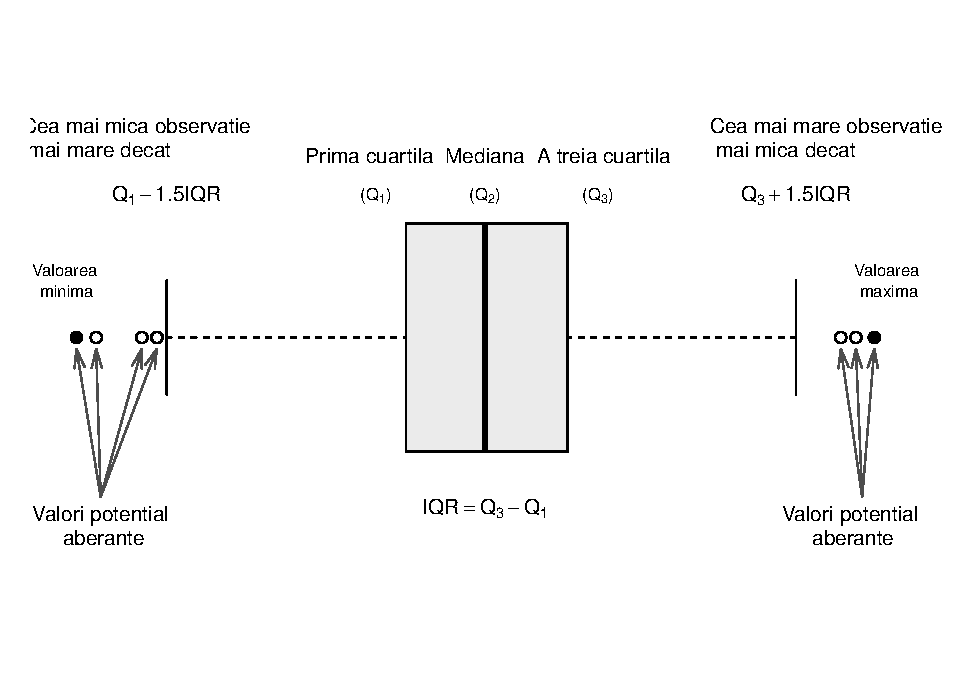
\includegraphics[width=0.7\linewidth]{Lab_2_files/figure-latex/unnamed-chunk-27-1} \end{center}

În R metoda grafică boxplot se poate trasa cu ajutorul funcției
\texttt{boxplot()}. Aceasta primește ca argumente sau un vector de
observații numerice \texttt{x} atunci când dorim să ilustrăm repartiția
unei variabile sau o formulă de tipul \texttt{y\textasciitilde{}grup},
unde \texttt{y} este un vector numeric care va fi împărțit în funcție de
variabila discretă \texttt{grup}, atunci când vrem să comparăm aceeași
variabilă numerică în funcție de una discretă (calitatăvă). Pentru mai
multe informații tastați \texttt{?boxplot}.

\begin{rmdexercise}
Considerați setul de date \texttt{mtcars}. Investigați cu ajutorul unui
boxplot cum variază greutatea mașinilor, variabila \texttt{wt}, în
funcție de numărul de cilindrii \texttt{cyl}. Afișați numele mașinilor
care prezintă potențiale valori aberante. Aceeași cerință pentru
perechile \texttt{mpg} - \texttt{cyl}, \texttt{hp} - \texttt{cyl} și
\texttt{hp} - \texttt{am}.
\end{rmdexercise}

\begin{Shaded}
\begin{Highlighting}[]
\KeywordTok{par}\NormalTok{(}\DataTypeTok{bty =} \StringTok{"n"}\NormalTok{)}
\NormalTok{bp =}\StringTok{ }\KeywordTok{boxplot}\NormalTok{(mtcars}\OperatorTok{$}\NormalTok{wt }\OperatorTok{~}\StringTok{ }\NormalTok{mtcars}\OperatorTok{$}\NormalTok{cyl,}
             \DataTypeTok{xlab =} \StringTok{"Numar de cilindrii"}\NormalTok{, }
             \DataTypeTok{ylab =} \StringTok{"Greutate (in tone)"}\NormalTok{,}
             \DataTypeTok{col =} \StringTok{"grey80"}\NormalTok{,}
             \DataTypeTok{main =} \StringTok{"Setul de date mtcars: greutate vs numar cilindrii"}\NormalTok{)}

\NormalTok{cars =}\StringTok{ }\NormalTok{mtcars[mtcars}\OperatorTok{$}\NormalTok{cyl }\OperatorTok{==}\StringTok{ }\DecValTok{8}\NormalTok{, ]}
\NormalTok{cars.names =}\StringTok{ }\KeywordTok{rownames}\NormalTok{(cars)[}\KeywordTok{which}\NormalTok{(cars}\OperatorTok{$}\NormalTok{wt }\OperatorTok\StringTok{ }\NormalTok{bp}\OperatorTok{$}\NormalTok{out)]}

\KeywordTok{text}\NormalTok{(}\KeywordTok{c}\NormalTok{(}\DecValTok{3}\NormalTok{,}\DecValTok{3}\NormalTok{,}\FloatTok{2.4}\NormalTok{)}\OperatorTok{+}\FloatTok{0.3}\NormalTok{, bp}\OperatorTok{$}\NormalTok{out, cars.names, }\DataTypeTok{cex =} \FloatTok{0.6}\NormalTok{)}
\KeywordTok{text}\NormalTok{( }\KeywordTok{c}\NormalTok{(}\DecValTok{1}\OperatorTok{:}\KeywordTok{length}\NormalTok{(}\KeywordTok{unique}\NormalTok{(mtcars}\OperatorTok{$}\NormalTok{cyl))) , }
\NormalTok{      bp}\OperatorTok{$}\NormalTok{stats[}\KeywordTok{nrow}\NormalTok{(bp}\OperatorTok{$}\NormalTok{stats) , ] }\OperatorTok{+}\StringTok{ }\FloatTok{0.5}\NormalTok{ , }
      \KeywordTok{paste}\NormalTok{(}\StringTok{"n = "}\NormalTok{, }\KeywordTok{table}\NormalTok{(mtcars}\OperatorTok{$}\NormalTok{cyl),}\DataTypeTok{sep=}\StringTok{""}\NormalTok{),}
      \DataTypeTok{cex =} \FloatTok{0.8}\NormalTok{)}
\end{Highlighting}
\end{Shaded}

\begin{center}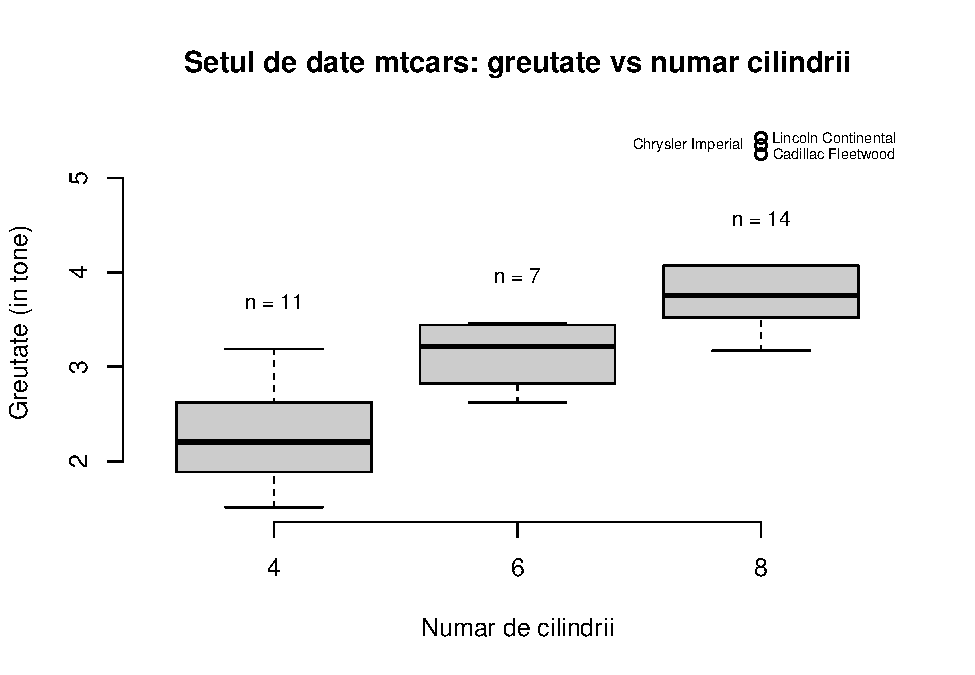
\includegraphics[width=0.7\linewidth]{Lab_2_files/figure-latex/unnamed-chunk-29-1} \end{center}

Numele mașinilor care au o greutate potențial aberantă este Cadillac
Fleetwood, Lincoln Continental, Chrysler Imperial.

\begin{rmdexercise}
Considerați setul de date \texttt{chickwts}. Investigați cu ajutorul
unui boxplot cum variază greutatea găinilor, variabila \texttt{weight},
în funcție de tipul de alimentație \texttt{feed}.
\end{rmdexercise}

\begin{center}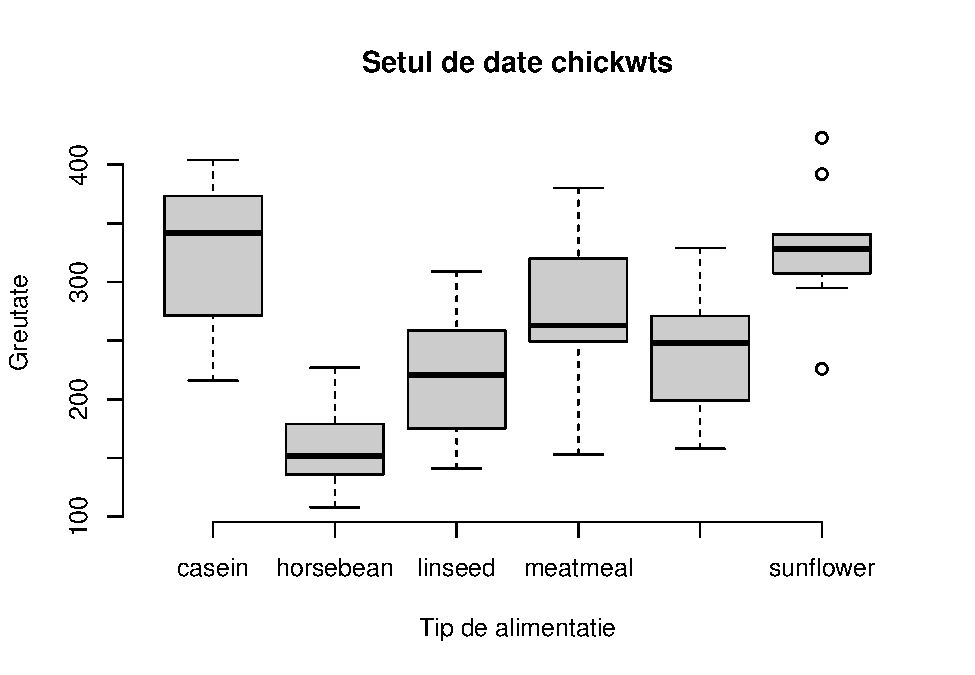
\includegraphics[width=0.7\linewidth]{Lab_2_files/figure-latex/unnamed-chunk-31-1} \end{center}

\section*{Referințe}\label{referinte}
\addcontentsline{toc}{section}{Referințe}

\hypertarget{refs}{}
\hypertarget{ref-FreedmanDiaconis1981}{}
Freedman, D., and P. Diaconis. 1981. ``On the Histogram as a Density
Estimator: \(L_2\) Theory.'' \emph{Z. Wahrscheinlichkeitstheorie Verw.
Gebiete} 57: 453--76.

\hypertarget{ref-Hyndman1996}{}
Hyndman, R. J., and Y Fan. 1996. ``Sample Quantiles in Statistical
Packages.'' \emph{American Statistician} 50: 361--65.

\hypertarget{ref-Tukey1977}{}
J., Tukey. 1977. \emph{Exploratory Data Analysis}. Addison-Wesley
Publishing Company.

\hypertarget{ref-Scott1979}{}
Scott, D. 1979. ``On Optimal and Data-Based Histograms.''
\emph{Biometrika} 66: 605--10.

\hypertarget{ref-Sturges1926}{}
Sturges, H. 1926. ``The Choice of a Class Interval.'' \emph{Journal of
the American Statistical Association} 65.


\end{document}
